\documentclass[tikz,border=2pt]{standalone}
\usepackage{amsmath,amssymb}
\usepackage{pgfplots}
\pgfplotsset{compat=1.18}
\usetikzlibrary{calc}

\begin{document}
% Joint density 2 on 0 < x < y < 1. Integrating along the vertical slice at x gives
% f_X(x) = 2(1 - x); along the horizontal slice at y gives f_Y(y) = 2y.
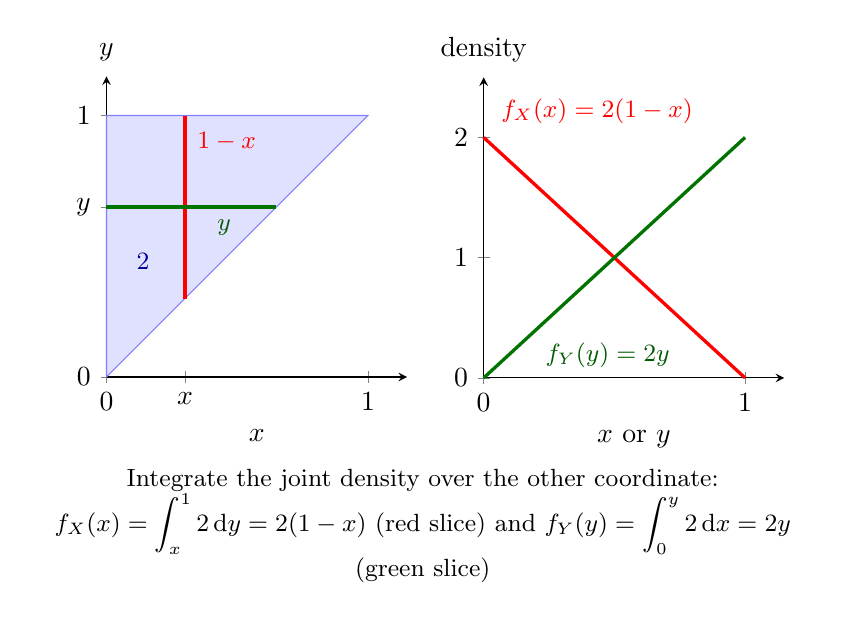
\begin{tikzpicture}
	\begin{axis}[
		name=joint, axis lines=left, xmin=0, xmax=1.15, ymin=0, ymax=1.15,
		xtick={0,0.3,1}, xticklabels={$0$,$x$,$1$}, ytick={0,0.65,1}, yticklabels={$0$,$y$,$1$},
		xlabel={$x$}, ylabel={$y$}, ylabel style={rotate=-90, anchor=south, at={(axis description cs:0,1.02)}},
		width=5.4cm, height=5.4cm, clip=false
		]
		\addplot[fill=blue!12, draw=blue!50] coordinates {(0,0) (1,1) (0,1)} -- cycle;
		\draw[red, very thick] (axis cs:0.3,0.3) -- (axis cs:0.3,1);
		\draw[green!45!black, very thick] (axis cs:0,0.65) -- (axis cs:0.65,0.65);
		\node[red, font=\small, anchor=west] at (axis cs:0.31,0.9) {$1-x$};
		\node[green!35!black, font=\small, anchor=north] at (axis cs:0.45,0.64) {$y$};
		\node[blue!60!black, font=\small] at (axis cs:0.14,0.44) {$2$};
	\end{axis}
	\begin{axis}[
		name=marg, at={(joint.outer east)}, anchor=outer west, xshift=3mm,
		axis lines=left, xmin=0, xmax=1.15, ymin=0, ymax=2.5,
		xtick={0,1}, ytick={0,1,2},
		xlabel={$x$ or $y$}, ylabel={density}, ylabel style={rotate=-90, anchor=south, at={(axis description cs:0,1.02)}},
		width=5.4cm, height=5.4cm, clip=false
		]
		\addplot[red, very thick, domain=0:1] {2*(1-x)};
		\addplot[green!45!black, very thick, domain=0:1] {2*x};
		\node[red, font=\small, anchor=south west] at (axis cs:0.03,2.03) {$f_X(x)=2(1-x)$};
		\node[green!35!black, font=\small, anchor=south west] at (axis cs:0.2,0.0) {$f_Y(y)=2y$};
	\end{axis}
	\node[anchor=north, font=\small, align=flush center, text width=9.8cm] at ([yshift=-2pt]$(joint.outer south)!0.5!(marg.outer south)$) {Integrate the joint density over the other coordinate: $f_X(x)=\displaystyle\int_x^12\,\mathrm{d}y=2(1-x)$ (red slice) and $f_Y(y)=\displaystyle\int_0^y2\,\mathrm{d}x=2y$ (green slice)};
\end{tikzpicture}
\end{document}
